% A complete fritzing circuit with all the wiring of the different sensors, actuators and components for display
% + A detailed explanation of your wiring choices as well as any additional technical choices (power, use of resistors, diodes, etc.)
% + A detailed explanation of the chosen components role and operating principle
\section{Électronique}

\subsection{Choix des composants}

Le choix des composants a été une étape importante dans la réalisation de notre robot.

Voici les différents composants que nous avons utilisés :
\begin{itemize}
    \item L293D : Un pont en H, pour contrôler nos moteurs.
    \item 1602A : Un écran LCD, pour afficher des informations sur notre robot.
    \item PCF8574T : Pour contrôler notre écran LCD à travers le bus I2C permettant d'économiser des pins sur notre Raspberry Pi.
    \item SJ-GU-TF-Luna : Un capteur de distance LIDAR pour détecter les obstacles, ce capteur est plus précis que le capteur de distance à ultrasons.
    \item MAX 98357A : Un convertisseur numérique vers analogique I2S et amplificateur de puissance de classe D pour contrôler notre haut-parleur.
    \item Un haut-parleur pour émettre des sons.
    \item Joy-it RB-CAMERA-JT (basé sur un OV5647) : Un caméra pour repérer la position de la ligne.
    \item Une batterie externe pour alimenter notre Raspberry Pi et la logique de notre robot.
    \item Un pack de 2 batteries lithium-ion 18650 pour alimenter nos moteurs.
\end{itemize}

Ces composants on été choisis en fonction de plusieurs critères :
\begin{itemize}
    \item L'utilisation de bus de communication afin d'économiser des pins sur notre Raspberry Pi. C'est le cas pour l'écran LCD couplé avec le PCF8574T et le capteur de distance LIDAR qui utilise le bus I2C.
    \item Leur facilité d'utilisation. C'est le cas de la carte de développement L293D.
    \item Lié a des contraintes de support logiciel. C'est le cas du MAX 98357A car la sortie son du Raspberry Pi est mal supportée logiciellement.
    \item Leur disponibilité au laboratoire d'électronique.
\end{itemize}

\subsection{Câblage des composants}

\subsubsection*{Optimisation de notre câblage}
Nous avons porter une attention particulière à l'organisation interne de notre robot. Par exemple, nous avons 
\begin{itemize}
    \item Surélevé notre Raspberry afin d'éviter des courts circuits avec les vis situées sur notre chassis.
    \item Réfléchi à l'emplacement des différents composants.
    \item Choisi les câbles les plus courts possibles.
\end{itemize}
Cependant, les gains de places notables ont été possibles grâce à :
\begin{itemize}
    \item L'utilisation d'une caméra, avec une nappe spécifique, en tant que capteur pour notre suiveur de ligne.
    \item L'usage d'une bread board pour connecter sur les mêmes GPIO notre LIDAR et notre écran LCD, tous les deux fonctionnant avec le protocole I2C qui permet le multiplexage de plusieurs composants.
\end{itemize}

\subsubsection*{Travail de soudure}
Nous avons également réalisé un gros travail de soudure sur nos capteurs QTR avant leur remplacement. En effet, nous avions refait l'intégralité de leur cablâge à partir de connecteurs Dupont et de gaines thermorétractables. Ceci nous permettait d'avoir un câble fixe, résistant à nos manipulations régulières et optimisé pour notre robot.
\\
\\
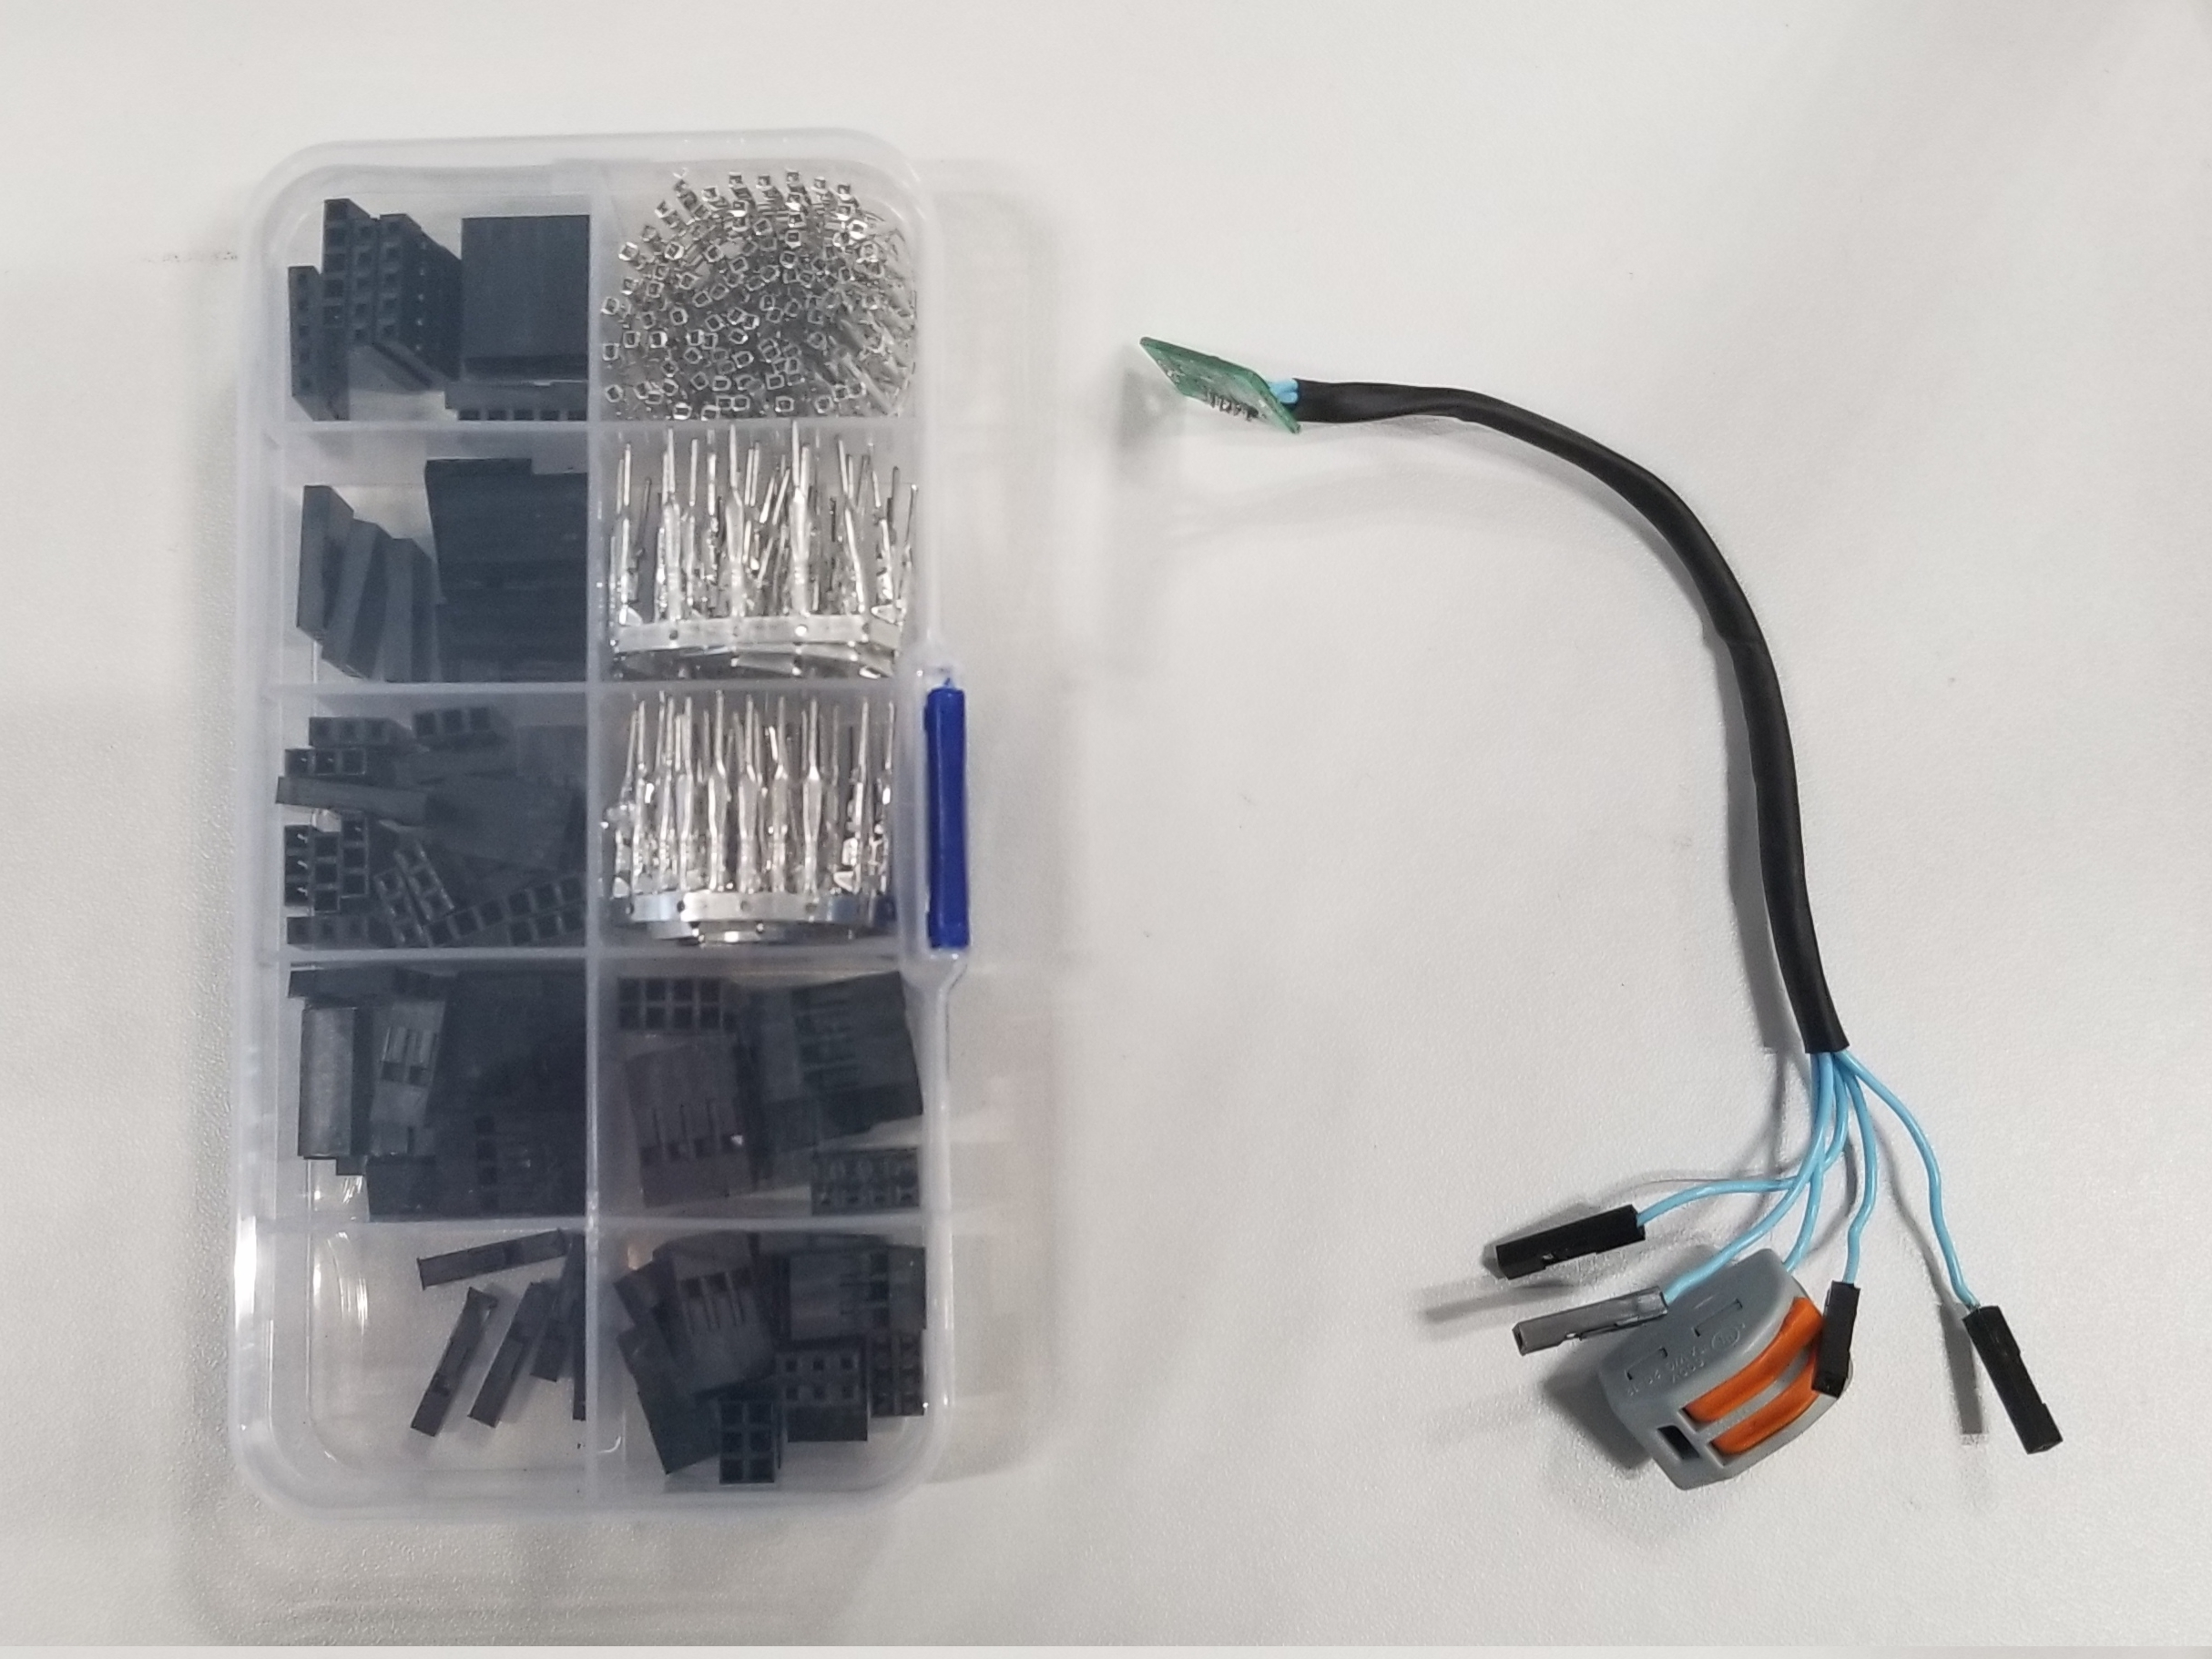
\includegraphics[scale=0.09]{../images/capteurQTR.jpg}

\subsection{Schéma électrique}

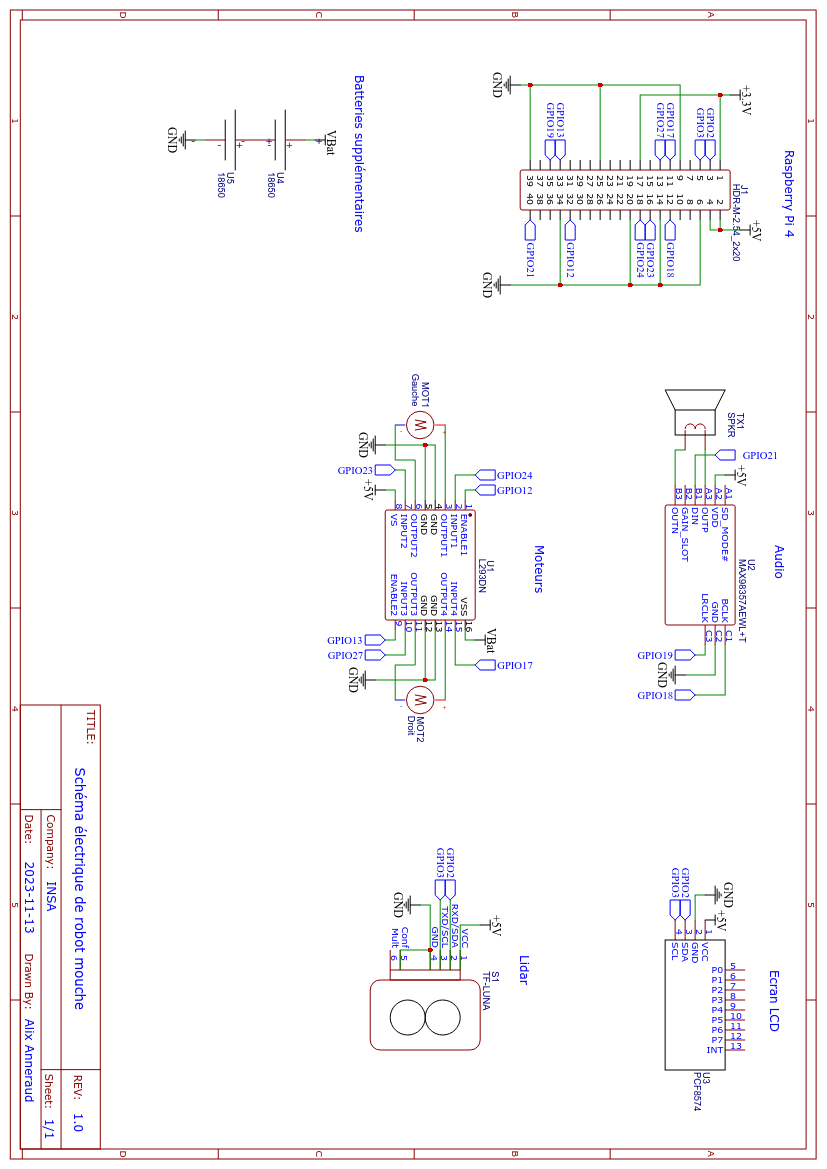
\includegraphics[scale=0.5]{../images/Schema EasyEDA Robot-Mouche.png}